
\centering
\captionsetup{type=figure}

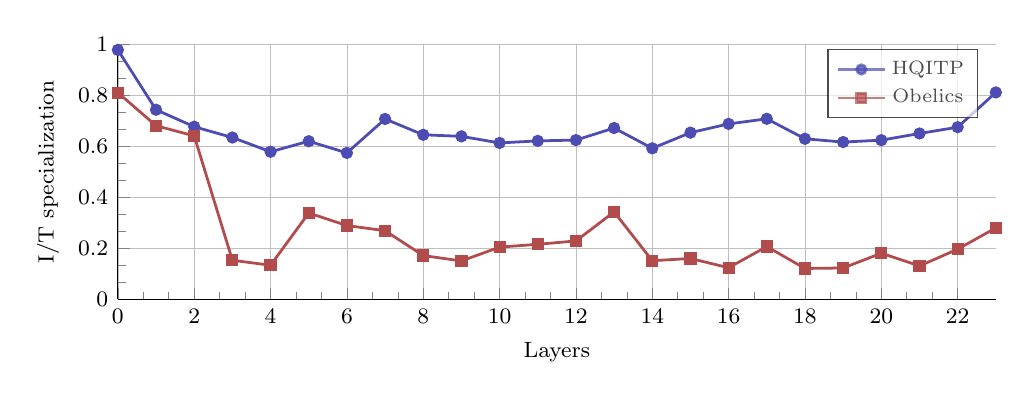
\begin{tikzpicture}
\begin{axis}[
    grid=major, %
    grid style={line width=.1pt, draw=gray!30}, %
    major grid style={line width=.2pt,draw=gray!50},
    minor tick num=2,
    axis x line*=bottom,
    axis y line*=left,
    xmin=0,
    xmax=23,
    ymin=0.0,
    ymax=1.0,
    height=1.9in,
    width=1.05\linewidth,
    ylabel style={align=center, font=\footnotesize},
    xlabel style={font=\footnotesize},
    ylabel=\footnotesize{I/T specialization},
    xlabel={\footnotesize{Layers}},
    ytick distance=0.2,
    yticklabel style={font=\footnotesize, /pgf/number format/fixed, /pgf/number format/precision=2},
    xticklabel style={font=\footnotesize},
    xtick={0,2,4,6,8,10,12,14,16,18,20,22},
    xticklabels={0,2,4,6,8,10,12,14,16,18,20,22},
    mark options={solid},
    legend style={cells={align=left}, font=\scriptsize, text=black, opacity=0.7}, %
]

\addplot[color=blue!40!gray, mark=*, mark size=1.7pt, line width=1pt] plot coordinates {  %
(0, 0.9769479348349329)
(1, 0.7427025603097698)
(2, 0.6762374582380828)
(3, 0.6340138224507533)
(4, 0.5783047019889138)
(5, 0.6195673358863271)
(6, 0.5737861572855565)
(7, 0.7066104505575633)
(8, 0.6446960774170309)
(9, 0.6386074080824291)
(10, 0.6128197724774395)
(11, 0.620867456928868)
(12, 0.6240480502092688)
(13, 0.6712385178771478)
(14, 0.591805441066985)
(15, 0.6531511085896324)
(16, 0.6873617200378165)
(17, 0.7072043647262733)
(18, 0.6290614078343542)
(19, 0.6162376387022552)
(20, 0.6237776803436119)
(21, 0.649774290665718)
(22, 0.6745086003424091)
(23, 0.810597818982423)
};
\addlegendentry{HQITP}

\addplot[color=red!40!gray, mark=square*, mark size=1.7pt, line width=1pt] plot coordinates { %
(0, 0.8098464848229123)
(1, 0.6803114998878562)
(2, 0.640428138604904)
(3, 0.15356616480436047)
(4, 0.13402442087930844)
(5, 0.33860156581505885)
(6, 0.2894806232076399)
(7, 0.269278406260023)
(8, 0.17195894943324286)
(9, 0.15091557473173656)
(10, 0.2050356661788283)
(11, 0.21603190628094793)
(12, 0.22923064654990588)
(13, 0.34291773221125066)
(14, 0.15175535984919586)
(15, 0.16059145647036643)
(16, 0.12438172525723101)
(17, 0.20722842981400202)
(18, 0.12145399323126793)
(19, 0.12335098001817868)
(20, 0.1811717532056517)
(21, 0.13129565163316004)
(22, 0.19701360887683683)
(23, 0.28035775702112686)
};
\addlegendentry{Obelics}
\end{axis}


\end{tikzpicture}

\caption{\textbf{MoE 特化。} 基于熵的图像/文本特化(见~\cref{sec:specialization})跨层次对于两个数据源:HQITP 和 Obelics。  
\edit{这两个来源表现出相似的趋势:得分在早期层下降,然后在最后几层再次上升。}}
\label{fig:tokens_specialization}
